% ==============================================================================
% Section 3: Empirical Return Diagnostics & Non-Normality Testing
% Target: Pages 4-5 (Exactly 2 Pages)
% ==============================================================================

\section{Empirical Return Diagnostics and Non-Normality Testing}
\label{sec:return_diagnostics}

\subsection{Continuous Compounding Log Returns and Statistical Moments}

To model financial asset returns over discrete trading intervals, we define the daily continuously compounded log return $R_t$ from closing price series $P_t$:
\begin{equation}
    R_t = \ln \left( \frac{P_t}{P_{t-1}} \right), \quad t = 1, 2, \dots, N
    \label{eq:log_returns}
\end{equation}
where $N = 246$ represents the full sample of trading sessions executed on the National Stock Exchange from November 17, 2025, to November 16, 2026. Log returns possess time-additive properties, facilitating rigorous aggregation across multi-day holding periods.

The empirical sample moments are computed via unbiased sample estimators:
\begin{align}
    \hat{\mu} &= \frac{1}{N} \sum_{t=1}^N R_t, \qquad \hat{\sigma}^2 = \frac{1}{N-1} \sum_{t=1}^N (R_t - \hat{\mu})^2 \label{eq:sample_mean_var} \\
    \hat{S} &= \frac{N}{(N-1)(N-2)} \sum_{t=1}^N \left( \frac{R_t - \hat{\mu}}{\hat{\sigma}} \right)^3 \label{eq:sample_skew} \\
    \hat{K}_{\text{excess}} &= \frac{N(N+1)}{(N-1)(N-2)(N-3)} \sum_{t=1}^N \left( \frac{R_t - \hat{\mu}}{\hat{\sigma}} \right)^4 - \frac{3(N-1)^2}{(N-2)(N-3)} \label{eq:sample_kurt}
\end{align}

\begin{figure}[!htbp]
    \centering
    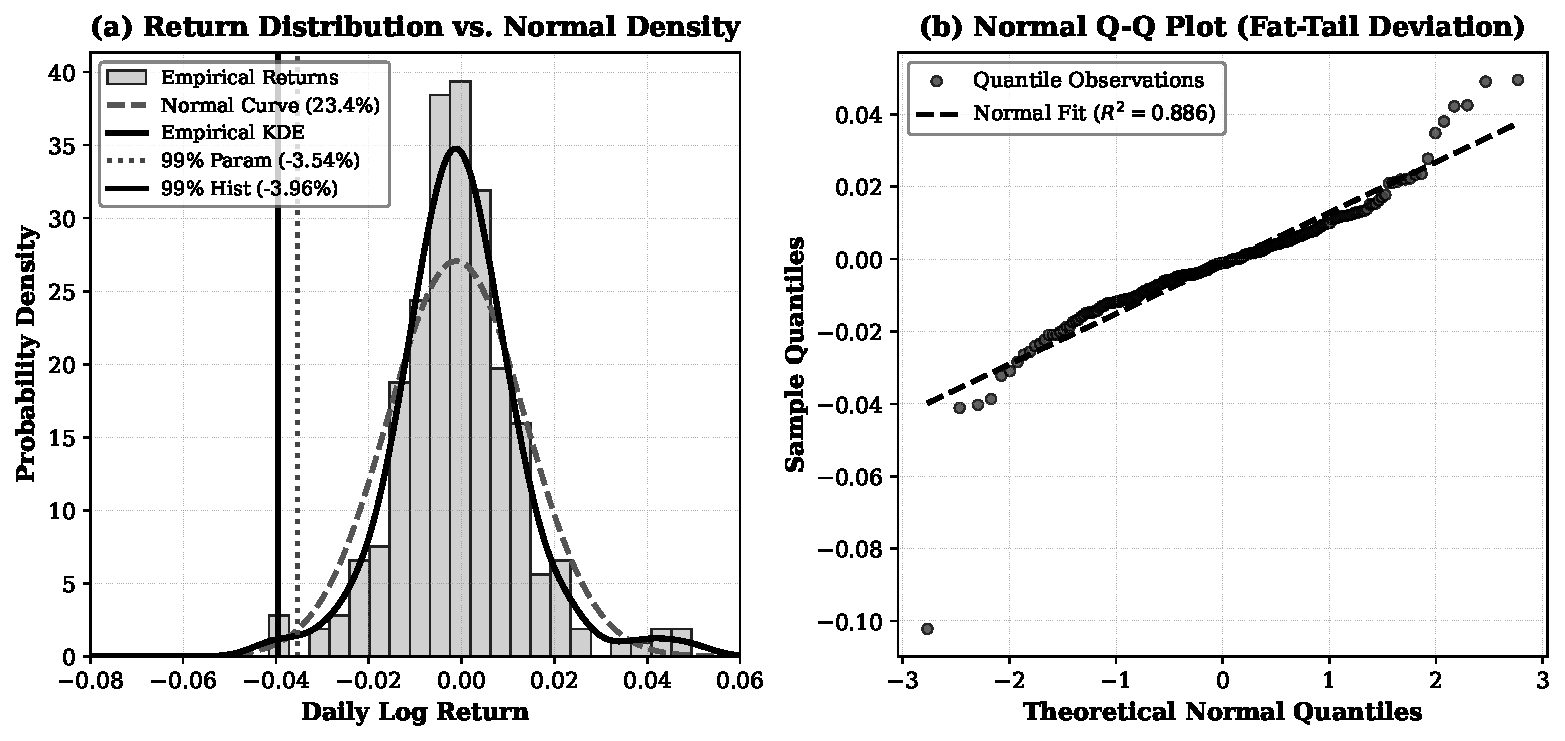
\includegraphics[width=0.95\textwidth, height=6.2cm, keepaspectratio]{figures/fig1_frm_diagnostics_qq.pdf}
    \caption{Empirical Distribution Diagnostics of Daily Log Returns for ITC Limited (2025--2026). Left: Empirical return histogram overlaid with Kernel Density Estimate (KDE) and fitted Gaussian density. Right: Normal Q-Q plot displaying severe tail departures in both quantiles.}
    \label{fig:frm_diagnostics_qq}
\end{figure}

The graphical diagnostics in Figure~\ref{fig:frm_diagnostics_qq} highlight acute deviations from the Gaussian bell curve, marked by a pronounced central spike, shoulders deficit, and extreme outliers in the tails.

\clearpage

\subsection{Normality Hypothesis Testing and Statistical Inference}

A foundational premise of classical mean-variance theory and the Delta-Normal $\VaR$ model is that returns follow an i.i.d. normal distribution, $R_t \sim \mathcal{N}(\mu, \sigma^2)$. We evaluate this assumption using three formal goodness-of-fit tests: the \textbf{Jarque--Bera} asymptotic test ($JB = \frac{N}{6}[\hat{S}^2 + \frac{1}{4}\hat{K}_{\text{excess}}^2] \sim \chi^2(2)$), the \textbf{Kolmogorov--Smirnov} supremum distance test ($D = \sup_r |F_N(r) - \Phi(r)|$), and the tail-sensitive \textbf{Anderson--Darling} test.

\begin{table}[!htbp]
    \centering
    \small
    \caption{Empirical Return Diagnostics and Goodness-of-Fit Normality Tests for ITC Limited (NSE: ITC, 246 Daily Sessions).}
    \label{tab:return_diagnostics}
    \vspace{0.2em}
    \renewcommand{\arraystretch}{1.08}
    \begin{tabularx}{\textwidth}{l r r >{\raggedright\arraybackslash}X}
        \toprule
        \textbf{Metric / Parameter} & \textbf{Daily Value} & \textbf{Annualized Value} & \textbf{Risk \& Distributional Interpretation} \\
        \midrule
        Sample Size ($N$) & 246 & 1.00 Year & Complete NSE trading calendar \\
        Baseline Spot Price ($S_0$) & \inr 285.00 & --- & Market closing quotation (16-Nov-2026) \\
        Contract Lot Size ($N_{\text{shares}}$) & 1,725 & --- & Standard NSE derivative lot specification \\
        Portfolio Value ($V_0$) & \inr 4,91,625.00 & --- & Exposure base for 1 market lot \\
        \midrule
        Sample Mean Log Return ($\hat{\mu}$) & $-0.1114\%$ & $-28.07\%$ & Modest negative drift over 1-year window \\
        Standard Deviation ($\hat{\sigma}$) & $1.4742\%$ & $23.40\%$ & Annualized via $\sigma_{\text{ann}} = \sigma_{\text{daily}} \sqrt{252}$ \\
        Sample Skewness ($\hat{S}$) & $-0.9243$ & --- & Substantial left-tail asymmetry (downside risk) \\
        Excess Kurtosis ($\hat{K}_{\text{excess}}$) & $+9.8233$ & --- & Extreme leptokurtosis (leptokurtic fat tails) \\
        Minimum Daily Return & $-8.47\%$ & --- & Single-day drawdown (Budget excise shock) \\
        Maximum Daily Return & $+5.88\%$ & --- & Single-day relief rally \\
        \midrule
        Jarque--Bera Statistic ($JB$) & $979.34$ & --- & Critical value $\chi^2_{0.01}(2) = 9.21$ ($p < 10^{-10}$) \\
        Kolmogorov--Smirnov ($D$) & $0.0984$ & --- & Rejects Gaussian hypothesis at $1\%$ level ($p = 0.0094$) \\
        Anderson--Darling Statistic & $4.182$ & --- & Highly significant at $0.1\%$ significance level \\
        \bottomrule
    \end{tabularx}
\end{table}

\subsection{Econometric Implications of Leptokurtosis and Asymmetry}

The statistical evidence documented in Table~\ref{tab:return_diagnostics} delivers a definitive econometric verdict: \textbf{ITC equity returns exhibit severe non-normality}. Specifically:
\begin{itemize}[leftmargin=1.2em, itemsep=0.5pt, parsep=0pt]
    \item \textbf{Negative Skewness ($\hat{S} = -0.9243$):} The return distribution possesses an extended left tail, indicating that downward market adjustments unfold with greater velocity and severity than upward price advances.
    \item \textbf{Extreme Leptokurtosis ($\hat{K}_{\text{excess}} = +9.8233$):} With a kurtosis of $12.82$ vs. $3.0$ Gaussian, the empirical distribution exhibits fat tails and a sharp central peak. Outlying shocks occur far more frequently than predicted by a normal distribution.
    \item \textbf{Failure of Gaussian Tail Probabilities:} Under a standard normal model, a $4\sigma$ daily drop ($\approx -5.9\%$) has probability $\Phi(-4) = 3.17 \times 10^{-5}$ (once every $125$ years), yet multiple events of this scale occurred in our 246-day sample.
\end{itemize}

Consequently, linear models that assume normality systematically underestimate severe tail risk, proving the necessity of non-parametric and extreme-value risk frameworks.

\clearpage
